\documentclass[tikz,border=10pt]{standalone}
\usepackage{tikz}
\usepackage{amsmath,amssymb}
\usetikzlibrary{positioning,shapes.geometric,arrows.meta,calc}

% Nature/Science style - minimal, professional
\definecolor{primary}{RGB}{31, 78, 121}
\definecolor{secondary}{RGB}{68, 114, 196}
\definecolor{accent}{RGB}{192, 80, 77}
\definecolor{neutral}{RGB}{127, 127, 127}
\definecolor{lightbg}{RGB}{248, 249, 250}
\definecolor{textdark}{RGB}{33, 37, 41}

\begin{document}
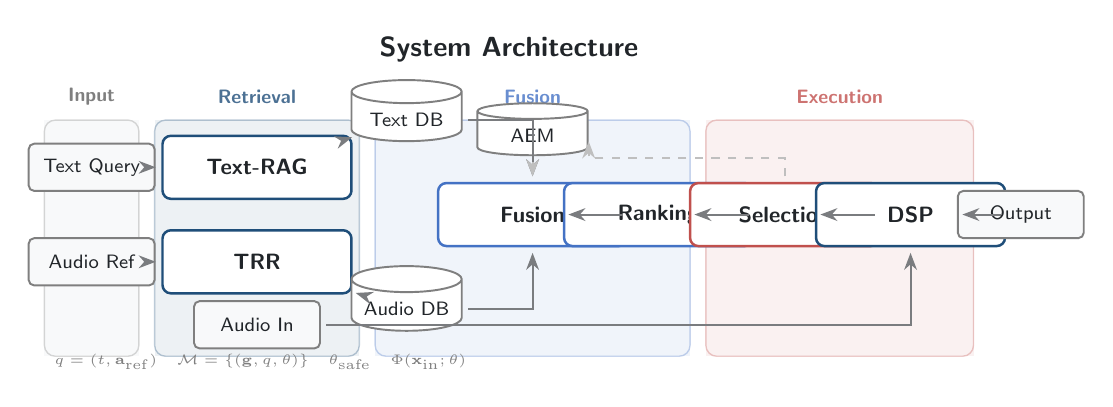
\begin{tikzpicture}[
    font=\sffamily\footnotesize,
    >=Stealth,
    thick,
    module/.style={
        rectangle, rounded corners=3pt,
        minimum width=2.4cm, minimum height=0.8cm,
        align=center,
        text=textdark,
        draw=#1, line width=0.9pt,
        fill=white
    },
    io/.style={
        rectangle, rounded corners=2pt,
        minimum width=1.6cm, minimum height=0.6cm,
        align=center,
        text=textdark,
        draw=neutral, line width=0.7pt,
        fill=lightbg,
        font=\sffamily\scriptsize
    },
    storage/.style={
        cylinder, shape border rotate=90, aspect=0.25,
        minimum width=1.4cm, minimum height=0.6cm,
        align=center,
        text=textdark,
        draw=neutral, line width=0.7pt,
        fill=white,
        font=\sffamily\scriptsize
    },
    flow/.style={
        ->, line width=0.7pt,
        color=textdark!60,
        shorten >=2pt, shorten <=2pt
    },
    grouplabel/.style={
        font=\sffamily\bfseries\scriptsize,
        text=neutral
    },
    bgbox/.style={
        rounded corners=4pt,
        line width=0.5pt,
        opacity=0.3
    }
]

% Background boxes first (no scope needed)
\fill[lightbg] (-0.6, 0.6) rectangle (0.6, -2.4);
\fill[primary!8] (0.8, 0.6) rectangle (3.4, -2.4);
\fill[secondary!8] (3.6, 0.6) rectangle (7.6, -2.4);
\fill[accent!8] (7.8, 0.6) rectangle (11.2, -2.4);

% Borders
\draw[bgbox, neutral] (-0.6, 0.6) rectangle (0.6, -2.4);
\draw[bgbox, primary] (0.8, 0.6) rectangle (3.4, -2.4);
\draw[bgbox, secondary] (3.6, 0.6) rectangle (7.6, -2.4);
\draw[bgbox, accent] (7.8, 0.6) rectangle (11.2, -2.4);

% Group labels
\node[grouplabel] at (0, 0.9) {Input};
\node[grouplabel, text=primary!80] at (2.1, 0.9) {Retrieval};
\node[grouplabel, text=secondary!80] at (5.6, 0.9) {Fusion};
\node[grouplabel, text=accent!80] at (9.5, 0.9) {Execution};

% COLUMN 1: Input
\node[io] at (0, 0) (textq) {Text Query};
\node[io] at (0, -1.2) (audioq) {Audio Ref};

% COLUMN 2: Encoding
\node[module={primary}] at (2.1, 0) (textrag) {\textbf{Text-RAG}};
\node[module={primary}] at (2.1, -1.2) (trr) {\textbf{TRR}};

% COLUMN 3: Knowledge Bases
\node[storage] at (4.0, 0.6) (textdb) {Text DB};
\node[storage] at (4.0, -1.8) (audiodb) {Audio DB};

% COLUMN 4: Fusion
\node[module={secondary}] at (5.6, -0.6) (fusion) {\textbf{Fusion}};

% COLUMN 5: Ranking
\node[module={secondary}] at (7.2, -0.6) (ranking) {\textbf{Ranking}};

% COLUMN 6: Selection
\node[module={accent}] at (8.8, -0.6) (selection) {\textbf{Selection}};

% COLUMN 7: DSP
\node[module={primary}] at (10.4, -0.6) (dsp) {\textbf{DSP}};

% COLUMN 8: Output
\node[io] at (11.8, -0.6) (output) {Output};

% Audio input at bottom
\node[io] at (2.1, -2.0) (audioin) {Audio In};

% Memory at top
\node[storage] at (5.6, 0.4) (memory) {AEM};

% === CONNECTIONS ===
\draw[flow] (textq) -- (textrag);
\draw[flow] (audioq) -- (trr);
\draw[flow] (textrag) -- (textdb);
\draw[flow] (trr) -- (audiodb);
\draw[flow] (textdb) -| (fusion);
\draw[flow] (audiodb) -| (fusion);
\draw[flow] (fusion) -- (ranking);
\draw[flow] (ranking) -- (selection);
\draw[flow] (selection) -- (dsp);
\draw[flow] (dsp) -- (output);
\draw[flow] (audioin) -| (dsp);

% Memory connections
\draw[flow, dashed, color=neutral!50] (memory) -- (fusion);
\draw[flow, dashed, color=neutral!50] (selection.north) -- ++(0,0.3) -| (memory.east);

% Math notation
\node[font=\sffamily\tiny, text=neutral, anchor=south west] at (-0.6, -2.7) {
    $q=(t,\mathbf{a}_{\mathrm{ref}})$ \quad $\mathcal{M}=\{(\mathbf{g},q,\theta)\}$ \quad $\theta_{\mathrm{safe}}$ \quad $\Phi(\mathbf{x}_{\mathrm{in}};\theta)$
};

% Title
\node[font=\sffamily\bfseries, text=textdark] at (5.3, 1.5) {System Architecture};

\end{tikzpicture}
\end{document}
